\chapter{လိုအပ်သည့် ဆော့ဖ်ဝဲများ ထည့်သွင်းခြင်း} \label{apdx1}

ဒီစာအုပ်မှာပါတဲ့ ဥပမာတွေကို လက်တွေ့စမ်းသပ် \fEn{run} ကြည့်ဖို့၊ လေ့ကျင့်ခန်းတွေ ပရောဂျက်တွေကို ပရိုဂရမ်လက်တွေ့ လိုက်ရေး လေ့ကျင့်နိုင်ဖို့အတွက် လိုအပ်တဲ့ ဆော့ဖ်ဝဲတွေ ထည့်ထားရပါမယ်။

\section*{Python နှင့် PyCharm IDE ထည့်သွင်းခြင်း}
ကွန်ပျူတာ ဆော့ဖ်ဝဲထည့်သွင်းတာ \fEn{(Software Installation)} အတွေ့အကြုံ ရှိထားပြီးသူတွေအတွက် အကျဉ်းချုံး အရင်ဖော်ပြပေးပါမယ်။ အတွေ့အကြုံ မရှိသေးတဲ့သူတွေအတွက်လည်း ဒါပြီးတဲ့အခါ တစ်ဆင့်ချင်းအသေးစိတ် ဆက်လက် ဖော်ပြပေးသွားမှာပါ။

\fCode{https://www.jetbrains.com/pycharm/download/} လင့်ကိုဖွင့်ပါ။ မိမိကွန်ပျူတာနဲ့ ကိုက်ညီတဲ့ \fEn{\mytcboxinl{PyCharm Community Edition}} ကို ဒေါင်းလုဒ်လုပ်ပြီး \fEn{install} လုပ်ပါ။ (ဝယ်သုံးရတဲ့ \fEn{\mytcboxinl{PyCharm Professional}} ကို ဒေါင်းလုဒ် မှားမလုပ်မိဖို့ သတိပြုပါ)။ ဒီစာရေးနေချိန် အခုလက်ရှိ ဗားရှင်းက ၂၀၂၃ ပါ။ သိပ်မကြာခင် ၂၀၂၄ ထွက်ပါတော့မယ်။ အကယ်၍ လက်ရှိဗားရှင်းထက် နိမ့်တဲ့ဗားရှင်းတွေကို ဒေါင်းလုဒ် လုပ်ချင်ရင် အောက်ပါ လင့်ကို သွားပါ။
%
\begin{minted}[frame=lines, framerule=0pt]{text}
https://www.jetbrains.com/pycharm/download/other.html
\end{minted}
%
\begin{mytcbox}
\noindent \qquad မှတ်ချက်။\qquad ။ ဗားရှင်း ၂၀၂၄/၂၅ ထွက်ပြီးတဲ့ အချိန်မှာ ၂၀၂၃ ဗားရှင်းကို လိုချင်ရင် အထက်ပါလင့်ကနေ ဒေါင်းလုဒ် လုပ်ပါ။ ၂၀၂၃ မှာလည်း ဗားရှင်းအခွဲတွေ ရှိပါသေးတယ်။ လက်ရှိအမြင့်ဆုံး ဗားရှင်းအခွဲ (ဥပမာ ၂၀၂၃.၃.၃) ကို သုံးလို့ရပါတယ်။ ၂၀၂၄/၂၅ သုံးမယ်ဆိုရင်လည်း ပြဿနာတော့ မရှိပါဘူး။ \fEn{Update} ဗားရှင်းဖြစ်တဲ့အတွက် ပုံတွေမှာ ပြထားတာနဲ့တော့ ကွာခြားချက်တချို့ ရှိကောင်းရှိနိုင်ပါတယ်။
\end{mytcbox}
%

အင်စတောလ်လုပ်ပြီးရင် \fEn{PyCharm IDE} ကိုဖွင့်ပြီး \fEn{New Project} နှိပ်ပြီး ပရောဂျက် အသစ်ယူပါ။ နံမည်ကို \fEn{MeetKarel} ပေးပါ။ ပုံ (\fRefNo{\ref{fig:new_proj}}) မှာ တွေ့ရတဲ့အတိုင်း \fEn{\mytcboxinl{Pure Python}, \mytcboxinl{Proj venv}} နဲ့ \fEn{Python} ဗားရှင်း \fEnBf{3.12.}\fEnEmpBf{xx} ကို ရွေးပါ။ \fEnEmpBf{xx} က အခြားဂဏန်း ဖြစ်နေနိုင်တယ်။ အဓိက ဗားရှင်း \fEn{3.12} သာ ဖြစ်ပါစေ။
\begin{figure}[tb!]
\begin{tikzpicture}
    \node[anchor=south west,inner sep=0] (image) at (0,0)
        {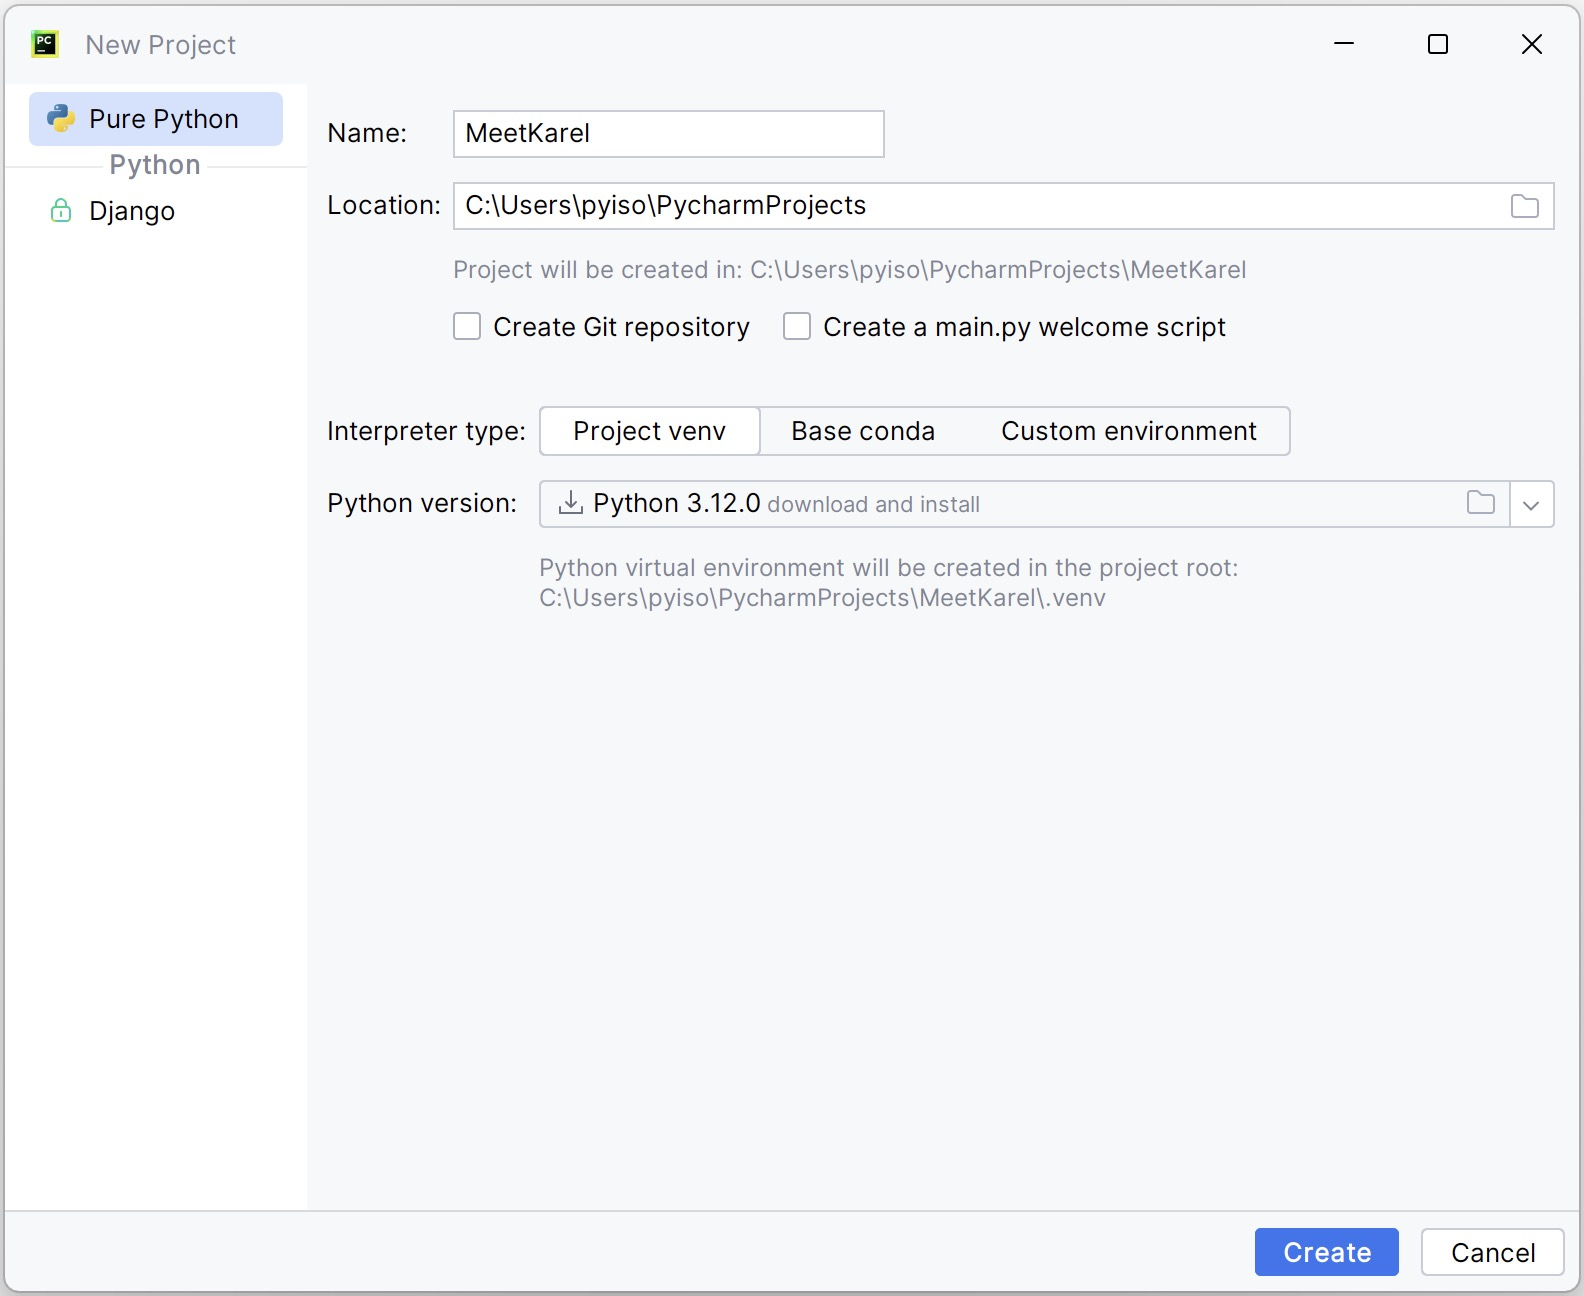
\includegraphics[width=.98\textwidth, trim={2.3mm 2mm 2mm 2.3mm},clip]{images/pycharm_install/new_proj.jpg}};
    \drawshadow{image}
    %\def\maxX{12}
    %\def\maxY{10}
    %\draw[step=.25,lightgray,ultra thin] (0,0) grid (\maxX,\maxY);
    %\draw[step=.5,gray,thin] (0,0) grid (\maxX, \maxY);
    %\draw[step=1,black,thin] (0,0) grid (\maxX, \maxY);
    %\foreach \x in {1,...,\maxX}
    %{
    %    \node at (\x,0) [below] {$\x$};
    %}
    %\foreach \y in {1,...,\maxY}
    %{
    %    \node at (0,\y) [left] {$\y$};
    %}

    \draw [draw=red,very thick,rounded corners] (0.15,9.82) rectangle (2.3,9.31);
    \draw [draw=red,very thick,rounded corners] (4.3,7.27) rectangle (6.21,6.76);
    \draw [draw=red,very thick,rounded corners] (4.3,6.68) rectangle (8,6.17);

\end{tikzpicture}
\caption{ပရောဂျက် အသစ်ယူခြင်း} 
\label{fig:new_proj}
\end{figure}

\begin{figure}[tb!]
\begin{tikzpicture}
    \node[anchor=south west,inner sep=0] (image) at (0,0)
        {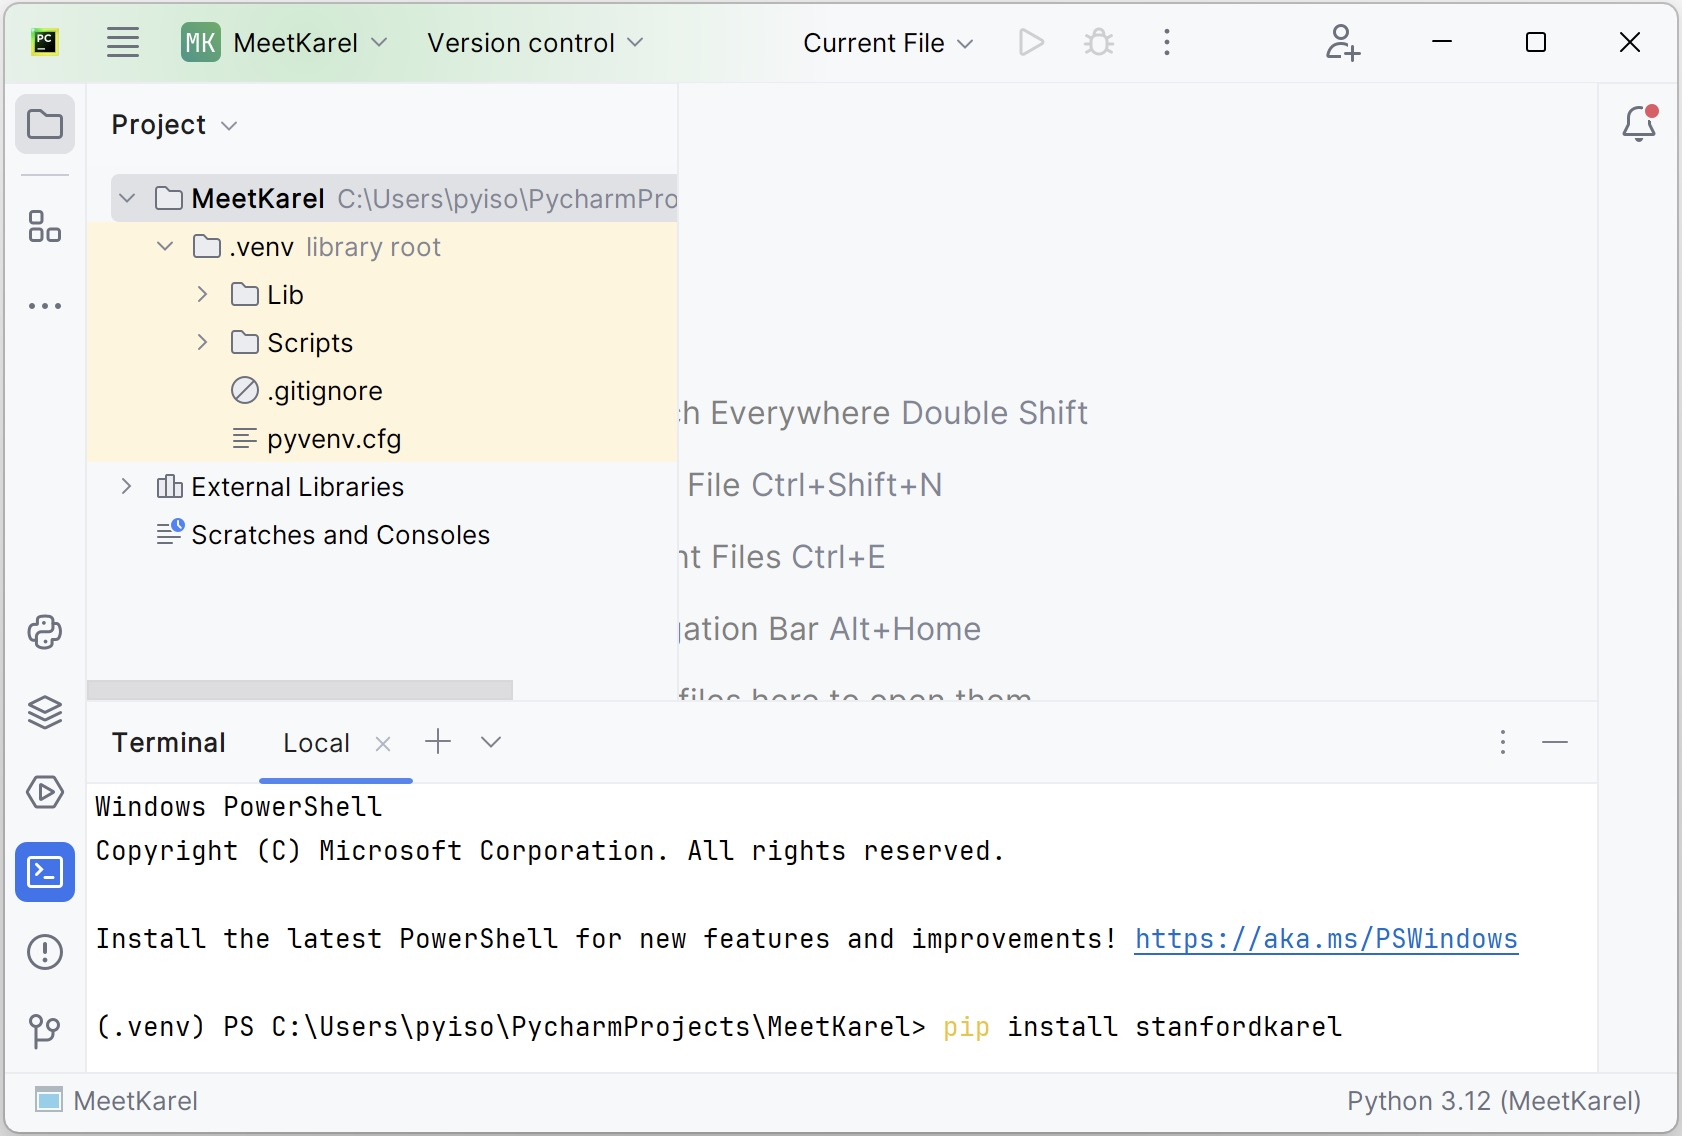
\includegraphics[width=.98\textwidth, trim={2.4mm 2mm 2mm 2.4mm},clip]{images/pycharm_install/install_karel.jpg}};
    \drawshadow{image}
    %\def\maxX{12}
    %\def\maxY{10}
    %\draw[step=.25,lightgray,ultra thin] (0,0) grid (\maxX,\maxY);
    %\draw[step=.5,gray,thin] (0,0) grid (\maxX, \maxY);
    %\draw[step=1,black,thin] (0,0) grid (\maxX, \maxY);
    %\foreach \x in {1,...,\maxX}
    %{
    %    \node at (\x,0) [below] {$\x$};
    %}
    %\foreach \y in {1,...,\maxY}
    %{
    %    \node at (0,\y) [left] {$\y$};
    %}

    \draw [draw=red,very thick,rounded corners] (0.02,2.26) rectangle (0.57,1.71);
    \draw [draw=red,very thick,rounded corners] (7.13,1.1) rectangle (10.4,0.55);

\end{tikzpicture}
\caption{Karel လိုက်ဘရီ အင်စတောလ်လုပ်ခြင်း} 
\label{fig:install_karel}
\end{figure}
ပုံ (\fRefNo{\ref{fig:install_karel}}) မှာ အနီရောင် ဝိုင်းပြထားတဲ့ အိုင်ကွန်ကို နှိပ်ပြီး \fEn{Terminal} ကိုဖွင့်ပါ။ \fEn{Terminal} မှာ အောက်ပါ ကွန်မန်းကို \fEn{run} ပြီး 
%
\begin{minted}[frame=lines, framerule=0pt]{text}
pip install stanfordkarel
\end{minted}
%
ကားရဲလ်လိုက်ဘရီကို အင်စတောလ်လုပ်ပါ။ ပုံ (\fRefNo{\ref{fig:install_karel}}) မှာ  အနီရောင် ဝိုင်းပြထားပါတယ်။ ခဏကြာတဲ့အခါ အခုလို \fOpn{မက်ဆေ့ချ်}တွေ ကျလာပါလိမ့်မယ်။ 

%
\begin{minted}[frame=lines, framerule=0pt,escapeinside=ßß]{text}
Collecting stanfordkarel
  Downloading stanfordkarel-0.2.7-py3-none-any.whl (51 kB)
     ━━━━━━━━━━━━━━━━━━━━━━━━━━━━━━━━━━━━━━━━ 51.9/51.9 kB 443.1 kB/s 
    eta 0:00:00
Installing collected packages: stanfordkarel
ß\colorbox{yellow}{Successfully installed stanfordkarel-0.2.7}ß

[notice] A new release of pip is available: 23.2.1 -> 24.0
[notice] To update, run: python.exe -m pip install --upgrade pip
(.venv) PS C:\Users\pyiso\PycharmProjects\MeetKarel>
\end{minted}
%
ဟိုက်လိုက်ပြထားတဲ့ \fOpn{မက်ဆေ့ချ်} တွေ့ရရင် အင်စတောလ်လုပ်တာ အောင်မြင်လို့ပါ။

\fEn{meet\_karel.zip} ဖိုင်ကို \todo{ဒေါင်းလုဒ်လင့်ထည့်ရန်} ဒီလင့် \fCode{http://tinyurl.com/3mmm9c7j} ကနေ ဒေါင်းလုဒ်လုပ်ပါ။ \fEn{meet\_karel.zip} ဖိုင်ကို \fEn{extract} လုပ်ပါ။ \fEn{meet\_karel} နံမည်နဲ့ ဖိုဒါတစ်ခု ရလာပါမယ်။ ၎င်းဖိုဒါထဲမှ အောက်ပါ \fEn{worlds} ဖိုဒါနှင့် \fEn{.py} ဖိုင်အားလုံးကို ကော်ပီလုပ်ပါ။ 
%
\begin{itemize}
    \item \fEn{worlds} 
    \item \fEn{meet\_karel.py}
    \item \fEn{move\_beeper\_to\_other\_side.py}
    \item \fEn{world\_editor.py}
\end{itemize}
%
\fEn{MeetKarel} ပရောဂျက်ထဲတွင် ကူးထည့်ပါ (ပင်မ ပရောဂျက် ဖိုဒါ ဖြစ်တဲ့ \fEn{MeetKarel} ဖိုဒါပေါ်မှာ ညာကလစ်နှိပ်ပြီး \fEn{Paste} လုပ်ရမှာပါ)။ ကော်ပီကူးထည့်လိုက်တဲ့ ဖိုင်တွေက ပုံ (\fRefNo{\ref{fig:proj_struct}}) မှာ တွေ့ရတဲ့အတိုင်း ဖြစ်သင့်ပါတယ်။

\fEn{meet\_karel.py} ဖိုင်ကို ကလစ်နှစ်ချက်နှိပ် ဖွင့်ပါ။ ပုံ (\fRefNo{\ref{fig:edit_meet_karel}}) မှာ တွေ့ရသလို ကုဒ်အယ်ဒီတာ \fEn{(code editor)} ပွင့်လာပါမယ်။ အောက်ပါအတိုင်း ဖြည့်စွက်ပါ။
%
\setlength{\fboxsep}{0pt}
\begin{minted}[frame=\mintframe, framerule=\mintrule,framesep= \mintsep, xleftmargin=\xlftmargin
                , bgcolor=mintbgcolor,rulecolor=mintrulecolor
                , python3=true]{python}
from stanfordkarel import *


def main():
    """Karel code goes here!"""
    move()
    move()
    move()
    pick_beeper()
    turn_left()
    move()
    move()

    turn_left()
    turn_left()
    turn_left()

    move()
    put_beeper()


if __name__ == "__main__":
    run_karel_program("meet_karel")
\end{minted}
%

%\fEn{lib, src, worlds} ဖိုဒါတို့ကို ပင်မ \fEn{project} ဖိုဒါအောက်မှာ ကော်ပီကူးထည့်ပါ။ \fEn{lib} ဖိုဒါကို \fEn{right click} နှိပ်ပြီး \fEn{Add as Library} လုပ်ပါ။ \fEn{src} ဖိုဒါထဲက \fEn{MeetKarel.java} ကိုဖွင့်ပြီး ပရိုဂရမ်ကို \fEn{run} ပါ။ ကားရဲလ် \fEn{Window} ပေါ်လာပါလိမ့်မယ်။ \fEn{Start Program} နှိပ်ရင် ကားရဲလ်က ဘိပါတုံးလေးကို နေရာရွှေ့ပေးပါလိမ့်မယ်။ (ပုံ \fRefNo{\ref{fig:proj_create01}} စာမျက်နှာ \fRefNo{\pageref{fig:proj_create01}} မှစ၍ \fRefNo{\ref{fig:proj_create13}} ထိ လိုအပ်ရင်ကြည့်ပါ)။ 

%http://tinyurl.com/3mmm9c7j
%https://bit.ly/42MhViS

% google drive root folder
%http://tinyurl.com/mkamnasm
%https://bit.ly/3T3tgrA



\fEn{meet\_karel.py} ဖိုင်ကို ညာကလစ်နှိမ်ပြီး \fEn{\mytcboxinl{Run 'meet\_karel'}} လုပ်ပါ။ ကားရဲလ် ပရိုဂရမ် ဝင်းဒိုး ပေါ်လာရင် \fEn{\mytcboxinl{Run Program}} ခလုပ်ကိုနှိပ်ပါ။ ကားရဲလ်ဟာ ပရိုဂရမ်ရေးထားတဲ့အတိုင်း လုပ်ဆောင်ပါလိမ့်မယ်။


\begin{figure}[tbh!]
\begin{tikzpicture}
    \node[anchor=south west,inner sep=0] (image) at (0,0)
        {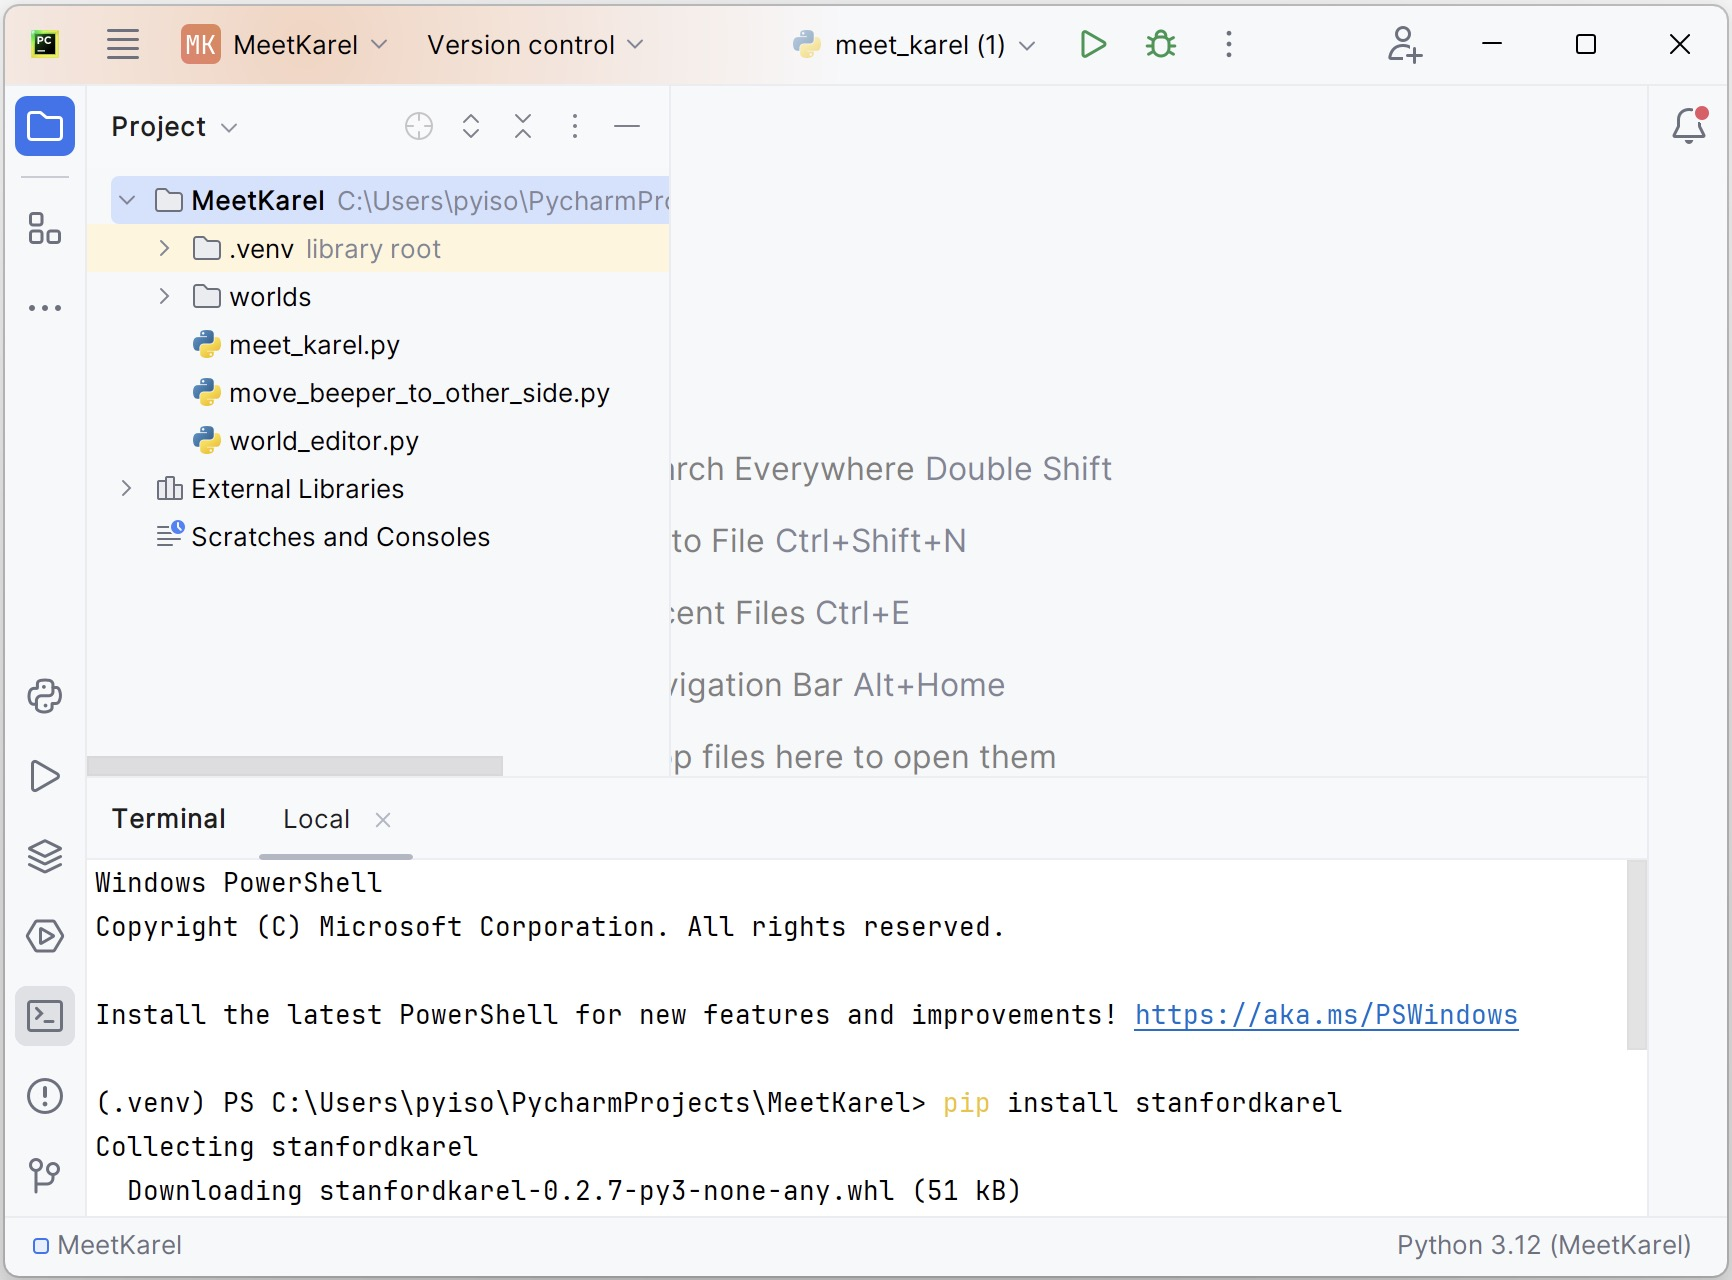
\includegraphics[width=.98\textwidth, trim={2.3mm 25cm 2mm 2.3mm},clip]{images/pycharm_install/folder_struct.jpg}};
    \drawshadow{image}
    %\def\maxX{12}
    %\def\maxY{10}
    %\draw[step=.25,lightgray,ultra thin] (0,0) grid (\maxX,\maxY);
    %\draw[step=.5,gray,thin] (0,0) grid (\maxX, \maxY);
    %\draw[step=1,black,thin] (0,0) grid (\maxX, \maxY);
    %\foreach \x in {1,...,\maxX}
    %{
    %    \node at (\x,0) [below] {$\x$};
    %}
    %\foreach \y in {1,...,\maxY}
    %{
    %    \node at (0,\y) [left] {$\y$};
    %}

    %\draw [draw=red,very thick,rounded corners] (0.15,9.82) rectangle (2.3,9.31);
    %\draw [draw=red,very thick,rounded corners] (4.3,7.27) rectangle (6.21,6.76);
    %\draw [draw=red,very thick,rounded corners] (4.3,6.68) rectangle (8,6.17);

\end{tikzpicture}
\caption{} 
\label{fig:proj_struct}
\end{figure}

\begin{figure}[tb!]
\begin{tikzpicture}
    \node[anchor=south west,inner sep=0] (image) at (0,0)
        {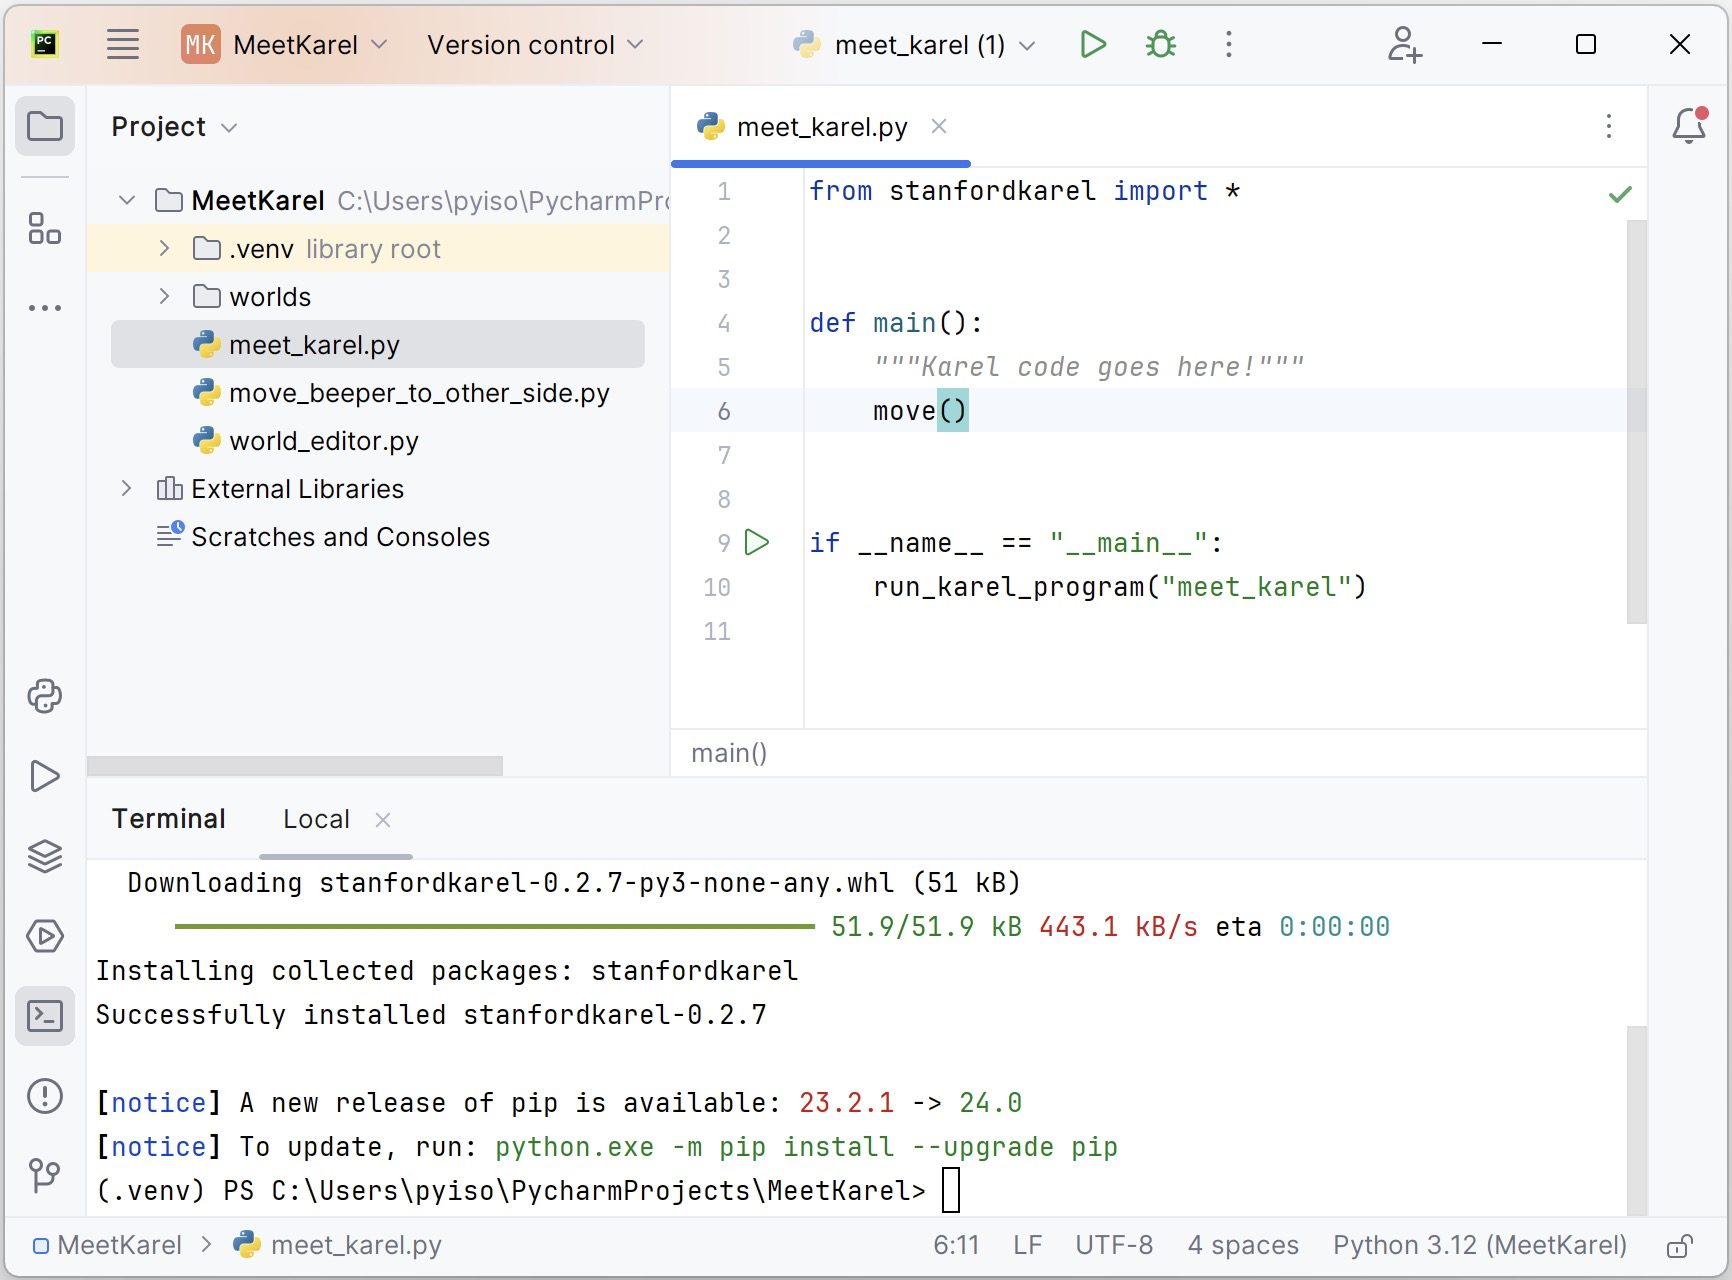
\includegraphics[width=.98\textwidth, trim={2.4mm 2mm 2mm 2.4mm},clip]{images/pycharm_install/edit_meet_karel.jpg}};
    \drawshadow{image}
    %\def\maxX{12}
    %\def\maxY{10}
    %\draw[step=.25,lightgray,ultra thin] (0,0) grid (\maxX,\maxY);
    %\draw[step=.5,gray,thin] (0,0) grid (\maxX, \maxY);
    %\draw[step=1,black,thin] (0,0) grid (\maxX, \maxY);
    %\foreach \x in {1,...,\maxX}
    %{
    %    \node at (\x,0) [below] {$\x$};
    %}
    %\foreach \y in {1,...,\maxY}
    %{
    %    \node at (0,\y) [left] {$\y$};
    %}



\end{tikzpicture}
\caption{} 
\label{fig:edit_meet_karel}
\end{figure}


%\fEn{MeetKarel.zip} ကို \todo{ဒေါင်းလုဒ်လင့်ထည့်ရန်} ဒီ \fCode{https://tinyurl.com/yesz8a6j} လင့်ကနေ ဒေါင်းလုဒ်လုပ်၊ \fEn{extract} လုပ်ပြီး \fEn{lib, src, worlds} ဖိုဒါတို့ကို ပင်မ \fEn{project} ဖိုဒါအောက်မှာ ကော်ပီကူးထည့်ပါ။ \fEn{lib} ဖိုဒါကို \fEn{right click} နှိပ်ပြီး \fEn{Add as Library} လုပ်ပါ။ \fEn{src} ဖိုဒါထဲက \fEn{MeetKarel.java} ကိုဖွင့်ပြီး ပရိုဂရမ်ကို \fEn{run} ပါ။ ကားရဲလ် \fEn{Window} ပေါ်လာပါလိမ့်မယ်။ \fEn{Start Program} နှိပ်ရင် ကားရဲလ်က ဘိပါတုံးလေးကို နေရာရွှေ့ပေးပါလိမ့်မယ်။ (ပုံ \fRefNo{\ref{fig:proj_create01}} စာမျက်နှာ \fRefNo{\pageref{fig:proj_create01}} မှစ၍ \fRefNo{\ref{fig:proj_create13}} ထိ လိုအပ်ရင်ကြည့်ပါ)။ 